\section{Gramáticas livre de contexto}

\begin{frame}[fragile]{Gramática livre de contexto}

    \begin{block}{Definição}
        Uma gramática livre de contexto é composta por terminais, não-terminais, um símbolo de partida e produções, onde
        \begin{enumerate}
            \item os terminais (tokens) são símbolos básicos para a formação de cadeias;
            \item os não-terminais são variáveis sintáticas que identificam cadeias de tokens e que impõem uma estrutura hierárquica na linguagem;
            \item um dentre os não-terminais é designado como símbolo de partida e o conjunto de cadeias geradas por ele é a linguagem definida pela gramática; e
            \item as produção estabelecem as relações entre terminais e não-terminais e como novas cadeias podem ser formadas. Cada produção é composta por um
                não-terminal seguido de uma seta, a qual é sucedida por uma cadeia de terminais e não-terminais.
        \end{enumerate}
    \end{block}

\end{frame}

\begin{frame}[fragile]{Convenções de notação}

    \begin{enumerate}
        \item São terminais:
            \begin{enumerate}[(i)]
                \item Letras minúsculas do alfabeto (por exemplo, $a, b, c, \ldots$)
                \item Simbolos de operadores (por exemplo, \code{apl}{+}, \code{apl}{-}, \code{apl}{×}, etc)
                \item Símbolos de pontuação, parêntesis, vírgulas, etc
                \item Os dígitos decimais \code{apl}{0}, \code{apl}{1}, \code{apl}{2}, ..., \code{apl}{9}
                \item Cadeias em negrito (por exemplo, \textbf{if}, \textbf{else}, \textbf{for}, etc)
            \end{enumerate}
        \pause

        \item São não-terminais:
            \begin{enumerate}[(i)]
                \item Letras maiúsculas do início do alfabeto (por exemplo, $A, B, C, \ldots$
                \item A letra $S$, em geral indicado o símbolo de partida
                \item Nomes em itálico formados por letras minúculas (por exemplo, $cmd$ e $expr$)
            \end{enumerate}
        \pause

        \item Letras maiúsculas do final do alfabeto ($X, Y, Z$) representam símbolos gramaticais, isto é, terminais ou não-terminais
    \end{enumerate}

\end{frame}

\begin{frame}[fragile]{Convenções de notação}

    \begin{enumerate}
        \setcounter{enumi}{3}
        \item Letras minúsculas do fim do alfabeto ($x, y, z$) representam cadeias de terminais
        \pause

        \item Letras gregas minúsculas (por exemplo, $\alpha, \beta, \gamma, \ldots$) representam cadeias de símbolos gramaticais (por exemplo, $A\to \alpha$ seria
            uma produção)
        \pause

        \item Se $A\to \alpha_1, A\to \alpha_2, \ldots A\to \alpha_N$ são produções com $A$ à esquerda (denominadas produções-$A$) então estas produções podem
            ser grafadas em uma só linha como
            \[
                A\to \alpha_1\ |\ \alpha_2\ |\ \ldots \ |\ \alpha_N,
            \]
            sendo cada $\alpha_i$ uma alternativa para $A$
        \pause

        \item O lado esquerdo da primeira produção é o símbolo de partida, salvo indicação contrária
    \end{enumerate}

\end{frame}

\begin{frame}[fragile]{Exemplo de gramática sem e com as convenções de notação}

\[
    \begin{array}{lp{2cm}l}
        expr \to expr\ op\ expr & \hspace{2in} & E \to E\ A\ E\ |\ (E)\ |\ \code{apl}{-}\ E\ |\ \textbf{id} \\
        expr \to (expr) & & A\to \code{apl}{+}\ |\ \code{apl}{-}\ |\ \code{apl}{×}\ |\ \code{apl}{÷}\ |\ \uparrow \\
        expr \to \code{apl}{-}\ expr \\
        expr \to \textbf{id} \\
        op \to\ \code{apl}{+} \\
        op \to\ \code{apl}{-} \\
        op \to\ \code{apl}{×} \\
        op \to\ \code{apl}{÷} \\
        op \to\ \uparrow
    \end{array}
\]

\end{frame}

\begin{frame}[fragile]{Derivações}

    \begin{block}{Definição de derivação}
        Seja $E$ um não-terminal, $E\to \alpha_1\ |\ \alpha_2\ |\ \ldots \ |\ \alpha_N$ produções-$E$ e $\sigma = \beta\ E\ \gamma$. É dito que $\sigma$ deriva 
            $\beta\ \alpha_i\ \gamma$, e notamos $\sigma \Rightarrow \beta\ \alpha_i\ \gamma$, se uma das instâncias de $E$ em $\sigma$ é substituída por uma
            das alternativas $\alpha_i$ das produções-$E$.

        \vspace{0.1in}

        Uma sequência de substituições em $\sigma$ que resulte em $X$ é chamada derivação de $X$ a partir de $\sigma$.
    \end{block}

\end{frame}

\begin{frame}[fragile]{Derivações em zero ou mais passos}

    \begin{block}{Definição em zero ou mais passos}
        Se $\alpha_1 \Rightarrow \alpha_2 \Rightarrow \ldots \Rightarrow \alpha_n$, então $\alpha_1$ deriva $\alpha_N$. O símbolo $\Rightarrow$ significa
        ``deriva em um passo''. O símbolo $\overset{\scalebox{0.5}{*}}{\Rightarrow}$ significa ``deriva em zero ou mais passos'' e o símbolo  $\overset{\scalebox{0.5}{+}}{\Rightarrow}$ significa
        ``deriva em um ou mais passos''.
    
        \vspace{0.1in}

        A derivação em zero ou mais passos tem duas importantes propriedades:
        \begin{enumerate}
            \item $\alpha \overset{\scalebox{0.5}{*}}{\Rightarrow} \alpha$ para qualquer cadeia $\alpha$, e
            \item se $\alpha \overset{\scalebox{0.5}{*}}{\Rightarrow} \beta$ e $\beta \overset{\scalebox{0.5}{*}}{\Rightarrow} \gamma$, então $\alpha \overset{\scalebox{0.5}{*}}{\Rightarrow} \gamma$ 
        \end{enumerate}
    \end{block}

\end{frame}

\begin{frame}[fragile]{Exemplo de derivação da expressão $\code{apl}{-}(\textbf{id}\ \code{apl}{+}\ \textbf{id})\ \code{apl}{×}\ \textbf{id}$}

\[
    \begin{array}{rcl}
        E & \Rightarrow & E\ \code{apl}{×}\ E \\
          & \Rightarrow & \code{apl}{-}\ E\ \code{apl}{×}\ E\\
          & \Rightarrow & \code{apl}{-}\ (E)\ \code{apl}{×}\ E\\
          & \Rightarrow & \code{apl}{-}\ (E\ \code{apl}{+}\ E)\ \code{apl}{×}\ E\\
          & \Rightarrow & \code{apl}{-}\ (E\ \code{apl}{+}\ E)\ \code{apl}{×}\ \textbf{id}\\
          & \Rightarrow & \code{apl}{-}\ (\textbf{id}\ \code{apl}{+}\ E)\ \code{apl}{×}\ \textbf{id}\\
          & \Rightarrow & \code{apl}{-}\ (\textbf{id}\ \code{apl}{+}\ \textbf{id})\ \code{apl}{×}\ \textbf{id}
    \end{array}
\]

\end{frame}

\begin{frame}[fragile]{Linguagem gerada por $G$}

    \begin{block}{Definição}
        Seja $G$ uma gramática e $S$ um símbolo de partida. O conjunto $L(G)$, denominado linguagem gerada por $G$, contém uma cadeia $w$ se, e somente se,
            $w$ contém apenas terminais e 
            $S \overset{\scalebox{0.5}{+}}{\Rightarrow} w$. A cadeia $w$ é denominada uma sentença de $G$. Uma linguagem que pode ser gerada por uma gramática é
            chamada linguagem livre de contexto.

            \vspace{0.1in}

            Se duas gramaticas $G_1$ e $G_2$ geram a mesma linguagem, então $G_1$ e $G_2$ são ditas equivalentes.

            \vspace{0.1in}

            Se $S \overset{\scalebox{0.5}{*}}{\Rightarrow} \alpha$, onde $\alpha$ pode conter tanto terminais quanto não-terminais e pode ser vazia, $\alpha$ é denominada uma forma sentencial de $G$.
    \end{block}

\end{frame}

\begin{frame}[fragile]{Árvores gramaticais e derivações}

    \begin{itemize}
        \item A ordem de substituição em uma derivação é arbitrária
        \pause

        \item Convém, portanto, assumir uma ordem de substituição, sendo as mais comuns substuir sempre o não-terminal mais à esquerda (gerando a forma sentencial
            mais à esquerda) ou mais à direita (derivações canônicas)
        \pause

        \item Uma árvore gramatical pode ser vista como uma representação gráfica de uma derivação que determine uma ordem de substituição
        \pause

        \item A ordem escolhida definirá o formato da árvore
        \pause

        \item Uma gramática que produz mais de uma árvore gramatical para alguma sentença é dita ambígua
    \end{itemize}

\end{frame}

\begin{frame}[fragile]{Árvore gramatical da derivação da expressão $\code{apl}{-}(\textbf{id}\ \code{apl}{+}\ \textbf{id})\ \code{apl}{×}\ \textbf{id}$}

    \begin{figure}
        \centering 

        \begin{tikzpicture}
            \node (A) at (6, 6) { $E$ };
        \end{tikzpicture}
    \end{figure}

\end{frame}

\begin{frame}[fragile]{Árvore gramatical da derivação da expressão $\code{apl}{-}(\textbf{id}\ \code{apl}{+}\ \textbf{id})\ \code{apl}{×}\ \textbf{id}$}

    \begin{figure}
        \centering 

        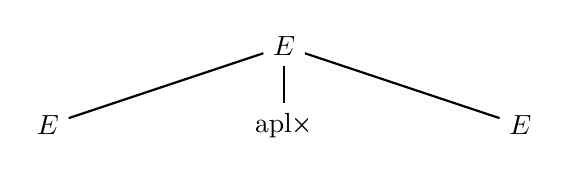
\begin{tikzpicture}
            \node (A) at (6, 6) { $E$ };

            \node (B1) at (3, 5) { $E$ };
            \node (B2) at (6, 5) { \code{apl}{×} };
            \node (B3) at (9, 5) { $E$ };
       
            \draw[thick] (A) to (B1); 
            \draw[thick] (A) to (B2); 
            \draw[thick] (A) to (B3); 
        \end{tikzpicture}
    \end{figure}

\end{frame}

\begin{frame}[fragile]{Árvore gramatical da derivação da expressão $\code{apl}{-}(\textbf{id}\ \code{apl}{+}\ \textbf{id})\ \code{apl}{×}\ \textbf{id}$}

    \begin{figure}
        \centering 

        \begin{tikzpicture}
            \node (A) at (6, 6) { $E$ };

            \node (B1) at (3, 5) { $E$ };
            \node (B2) at (6, 5) { \code{apl}{×} };
            \node (B3) at (9, 5) { $E$ };
       
            \draw[thick] (A) to (B1); 
            \draw[thick] (A) to (B2); 
            \draw[thick] (A) to (B3); 

            \node (C1) at (1, 4) { \code{apl}{-} };
            \node (C2) at (5, 4) { $E$ };
       
            \draw[thick] (B1) to (C1); 
            \draw[thick] (B1) to (C2); 

        \end{tikzpicture}
    \end{figure}

\end{frame}

\begin{frame}[fragile]{Árvore gramatical da derivação da expressão $\code{apl}{-}(\textbf{id}\ \code{apl}{+}\ \textbf{id})\ \code{apl}{×}\ \textbf{id}$}

    \begin{figure}
        \centering 

        \begin{tikzpicture}
            \node (A) at (6, 6) { $E$ };

            \node (B1) at (3, 5) { $E$ };
            \node (B2) at (6, 5) { \code{apl}{×} };
            \node (B3) at (9, 5) { $E$ };
       
            \draw[thick] (A) to (B1); 
            \draw[thick] (A) to (B2); 
            \draw[thick] (A) to (B3); 

            \node (C1) at (1, 4) { \code{apl}{-} };
            \node (C2) at (5, 4) { $E$ };
       
            \draw[thick] (B1) to (C1); 
            \draw[thick] (B1) to (C2); 

            \node (D1) at (4, 3) { \texttt{(} };
            \node (D2) at (5, 3) { $E$ };
            \node (D3) at (6, 3) { \texttt{)} };

            \draw[thick] (C2) to (D1); 
            \draw[thick] (C2) to (D2); 
            \draw[thick] (C2) to (D3); 

        \end{tikzpicture}
    \end{figure}

\end{frame}

\begin{frame}[fragile]{Árvore gramatical da derivação da expressão $\code{apl}{-}(\textbf{id}\ \code{apl}{+}\ \textbf{id})\ \code{apl}{×}\ \textbf{id}$}

    \begin{figure}
        \centering 

        \begin{tikzpicture}
            \node (A) at (6, 6) { $E$ };

            \node (B1) at (3, 5) { $E$ };
            \node (B2) at (6, 5) { \code{apl}{×} };
            \node (B3) at (9, 5) { $E$ };
       
            \draw[thick] (A) to (B1); 
            \draw[thick] (A) to (B2); 
            \draw[thick] (A) to (B3); 

            \node (C1) at (1, 4) { \code{apl}{-} };
            \node (C2) at (5, 4) { $E$ };
       
            \draw[thick] (B1) to (C1); 
            \draw[thick] (B1) to (C2); 

            \node (D1) at (4, 3) { \texttt{(} };
            \node (D2) at (5, 3) { $E$ };
            \node (D3) at (6, 3) { \texttt{)} };

            \draw[thick] (C2) to (D1); 
            \draw[thick] (C2) to (D2); 
            \draw[thick] (C2) to (D3); 

            \node (E1) at (4, 2) { $E$ };
            \node (E2) at (5, 2) { \code{apl}{+} };
            \node (E3) at (6, 2) { $E$ };

            \draw[thick] (D2) to (E1); 
            \draw[thick] (D2) to (E2); 
            \draw[thick] (D2) to (E3); 
        \end{tikzpicture}
    \end{figure}

\end{frame}

\begin{frame}[fragile]{Árvore gramatical da derivação da expressão $\code{apl}{-}(\textbf{id}\ \code{apl}{+}\ \textbf{id})\ \code{apl}{×}\ \textbf{id}$}

    \begin{figure}
        \centering 

        \begin{tikzpicture}
            \node (A) at (6, 6) { $E$ };

            \node (B1) at (3, 5) { $E$ };
            \node (B2) at (6, 5) { \code{apl}{×} };
            \node (B3) at (9, 5) { $E$ };
       
            \draw[thick] (A) to (B1); 
            \draw[thick] (A) to (B2); 
            \draw[thick] (A) to (B3); 

            \node (C1) at (1, 4) { \code{apl}{-} };
            \node (C2) at (5, 4) { $E$ };
            \node (C3) at (9, 4) { \textbf{id} };
       
            \draw[thick] (B1) to (C1); 
            \draw[thick] (B1) to (C2); 
            \draw[thick] (B3) to (C3); 

            \node (D1) at (4, 3) { \texttt{(} };
            \node (D2) at (5, 3) { $E$ };
            \node (D3) at (6, 3) { \texttt{)} };

            \draw[thick] (C2) to (D1); 
            \draw[thick] (C2) to (D2); 
            \draw[thick] (C2) to (D3); 

            \node (E1) at (4, 2) { $E$ };
            \node (E2) at (5, 2) { \code{apl}{+} };
            \node (E3) at (6, 2) { $E$ };

            \draw[thick] (D2) to (E1); 
            \draw[thick] (D2) to (E2); 
            \draw[thick] (D2) to (E3); 
        \end{tikzpicture}
    \end{figure}

\end{frame}

\begin{frame}[fragile]{Árvore gramatical da derivação da expressão $\code{apl}{-}(\textbf{id}\ \code{apl}{+}\ \textbf{id})\ \code{apl}{×}\ \textbf{id}$}

    \begin{figure}
        \centering 

        \begin{tikzpicture}
            \node (A) at (6, 6) { $E$ };

            \node (B1) at (3, 5) { $E$ };
            \node (B2) at (6, 5) { \code{apl}{×} };
            \node (B3) at (9, 5) { $E$ };
       
            \draw[thick] (A) to (B1); 
            \draw[thick] (A) to (B2); 
            \draw[thick] (A) to (B3); 

            \node (C1) at (1, 4) { \code{apl}{-} };
            \node (C2) at (5, 4) { $E$ };
            \node (C3) at (9, 4) { \textbf{id} };
       
            \draw[thick] (B1) to (C1); 
            \draw[thick] (B1) to (C2); 
            \draw[thick] (B3) to (C3); 

            \node (D1) at (4, 3) { \texttt{(} };
            \node (D2) at (5, 3) { $E$ };
            \node (D3) at (6, 3) { \texttt{)} };

            \draw[thick] (C2) to (D1); 
            \draw[thick] (C2) to (D2); 
            \draw[thick] (C2) to (D3); 

            \node (E1) at (4, 2) { $E$ };
            \node (E2) at (5, 2) { \code{apl}{+} };
            \node (E3) at (6, 2) { $E$ };

            \draw[thick] (D2) to (E1); 
            \draw[thick] (D2) to (E2); 
            \draw[thick] (D2) to (E3); 

            \node (F1) at (4, 1) { \textbf{id} };

            \draw[thick] (E1) to (F1); 
        \end{tikzpicture}
    \end{figure}

\end{frame}

\begin{frame}[fragile]{Árvore gramatical da derivação da expressão $\code{apl}{-}(\textbf{id}\ \code{apl}{+}\ \textbf{id})\ \code{apl}{×}\ \textbf{id}$}

    \begin{figure}
        \centering 

        \begin{tikzpicture}
            \node (A) at (6, 6) { $E$ };

            \node (B1) at (3, 5) { $E$ };
            \node (B2) at (6, 5) { \code{apl}{×} };
            \node (B3) at (9, 5) { $E$ };
       
            \draw[thick] (A) to (B1); 
            \draw[thick] (A) to (B2); 
            \draw[thick] (A) to (B3); 

            \node (C1) at (1, 4) { \code{apl}{-} };
            \node (C2) at (5, 4) { $E$ };
            \node (C3) at (9, 4) { \textbf{id} };
       
            \draw[thick] (B1) to (C1); 
            \draw[thick] (B1) to (C2); 
            \draw[thick] (B3) to (C3); 

            \node (D1) at (4, 3) { \texttt{(} };
            \node (D2) at (5, 3) { $E$ };
            \node (D3) at (6, 3) { \texttt{)} };

            \draw[thick] (C2) to (D1); 
            \draw[thick] (C2) to (D2); 
            \draw[thick] (C2) to (D3); 

            \node (E1) at (4, 2) { $E$ };
            \node (E2) at (5, 2) { \code{apl}{+} };
            \node (E3) at (6, 2) { $E$ };

            \draw[thick] (D2) to (E1); 
            \draw[thick] (D2) to (E2); 
            \draw[thick] (D2) to (E3); 

            \node (F1) at (4, 1) { \textbf{id} };
            \node (F2) at (6, 1) { \textbf{id} };

            \draw[thick] (E1) to (F1); 
            \draw[thick] (E3) to (F2); 
        \end{tikzpicture}
    \end{figure}

\end{frame}

\begin{frame}[fragile]{Duas derivações diferentes para a mesma expressão}

\[
    \begin{array}{rlp{2cm}rl}
        E & \Rightarrow E\ \code{apl}{+}\ E & & E & \Rightarrow E\ \code{apl}{×}\ E \\
        & \Rightarrow \textbf{id}\ \code{apl}{+}\ E & & & \Rightarrow E\ \code{apl}{+}\ E\ \code{apl}{×}\ E \\
        & \Rightarrow \textbf{id}\ \code{apl}{+}\ E\ \code{apl}{×}\ E & & & \Rightarrow \textbf{id}\ \code{apl}{+}\ E\ \code{apl}{×}\ E \\
        & \Rightarrow \textbf{id}\ \code{apl}{+}\ \textbf{id}\ \code{apl}{×}\ E & & & \Rightarrow \textbf{id}\ \code{apl}{+}\ \textbf{id}\ \code{apl}{×}\ E \\
        & \Rightarrow \textbf{id}\ \code{apl}{+}\ \textbf{id}\ \code{apl}{×}\ \textbf{id} & & & \Rightarrow \textbf{id}\ \code{apl}{+}\ \textbf{id}\ \code{apl}{×}\ \textbf{id} \\
    \end{array}
\]

\end{frame}

\begin{frame}[fragile]{Árvores sintáticas distintas que geram a mesma expressão}

    \begin{figure}
        \centering 

        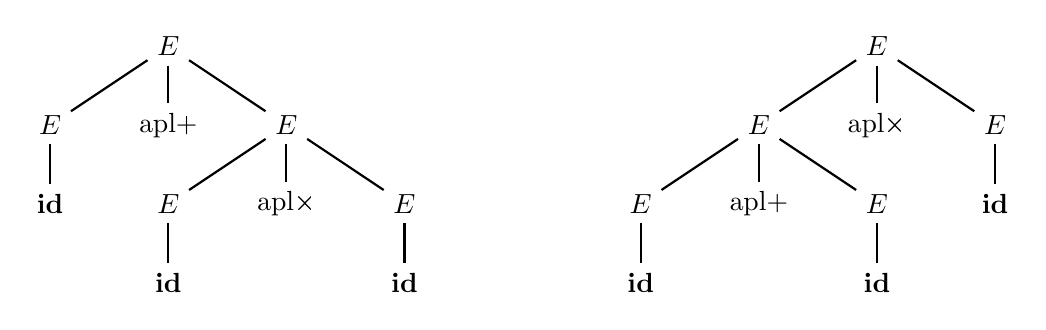
\begin{tikzpicture}
            \node (A) at (1.5, 6) { $E$ };
            \node (B1) at (0, 5) { $E$ };
            \node (B2) at (1.5, 5) { \code{apl}{+} };
            \node (B3) at (3, 5) { $E$ };
            \node (C1) at (0, 4) { \textbf{id} };
            \node (C2) at (1.5, 4) { $E$ };
            \node (C3) at (3, 4) { \code{apl}{×} };
            \node (C4) at (4.5, 4) { $E$ };
            \node (D1) at (1.5, 3) { \textbf{id} };
            \node (D2) at (4.5, 3) { \textbf{id} };

            \draw[thick] (A) to (B1);
            \draw[thick] (A) to (B2);
            \draw[thick] (A) to (B3);
            \draw[thick] (B1) to (C1);
            \draw[thick] (B3) to (C2);
            \draw[thick] (B3) to (C3);
            \draw[thick] (B3) to (C4);
            \draw[thick] (C2) to (D1);
            \draw[thick] (C4) to (D2);

            \node (X) at (10.5, 6) { $E$ };
            \node (Y1) at (9, 5) { $E$ };
            \node (Y2) at (10.5, 5) { \code{apl}{×} };
            \node (Y3) at (12, 5) { $E$ };
            \node (Z1) at (7.5, 4) { $E$ };
            \node (Z2) at (9, 4) { \code{apl}{+} };
            \node (Z3) at (10.5, 4) { $E$ };
            \node (Z4) at (12, 4) { \textbf{id} };
            \node (W1) at (7.5, 3) { \textbf{id} };
            \node (W2) at (10.5, 3) { \textbf{id} };

            \draw[thick] (X) to (Y1);
            \draw[thick] (X) to (Y2);
            \draw[thick] (X) to (Y3);
            \draw[thick] (Y1) to (Z1);
            \draw[thick] (Y1) to (Z2);
            \draw[thick] (Y1) to (Z3);
            \draw[thick] (Y3) to (Z4);
            \draw[thick] (Z1) to (W1);
            \draw[thick] (Z3) to (W2);
        \end{tikzpicture}
    \end{figure}

\end{frame}
